\chapter{Implementation}
% This chapter should describe what was actually produced: the programs which were written, the hardware which was built or the theory which was developed. Any design strategies that looked ahead to the testing stage might profitably be referred to (the professional approach again).
% Descriptions of programs may include fragments of high-level code but large chunks of code are usually best left to appendices or omitted altogether. Analogous advice applies to circuit diagrams.
% Draw attention to the parts of the work which are not your own. The Implementation Chapter should include a section labelled ”Repository Overview”. The repository overview should be around one page in length and should describe the high-level structure of the source code found in your source code Repository. It should describe whether the code was written from scratch or if it built on an existing project or tutorial. Making effective use of powerful tools and pre-existing code is often laudable, and will count to your credit if properly reported.
% It should not be necessary to give a day-by-day account of the progress of the work but major milestones may sometimes be highlighted with advantage.

%  ~4,500 words

% Tangent works better than correlation or partial correlation.
\section{Overview}

\begin{figure}[]
    \centering
    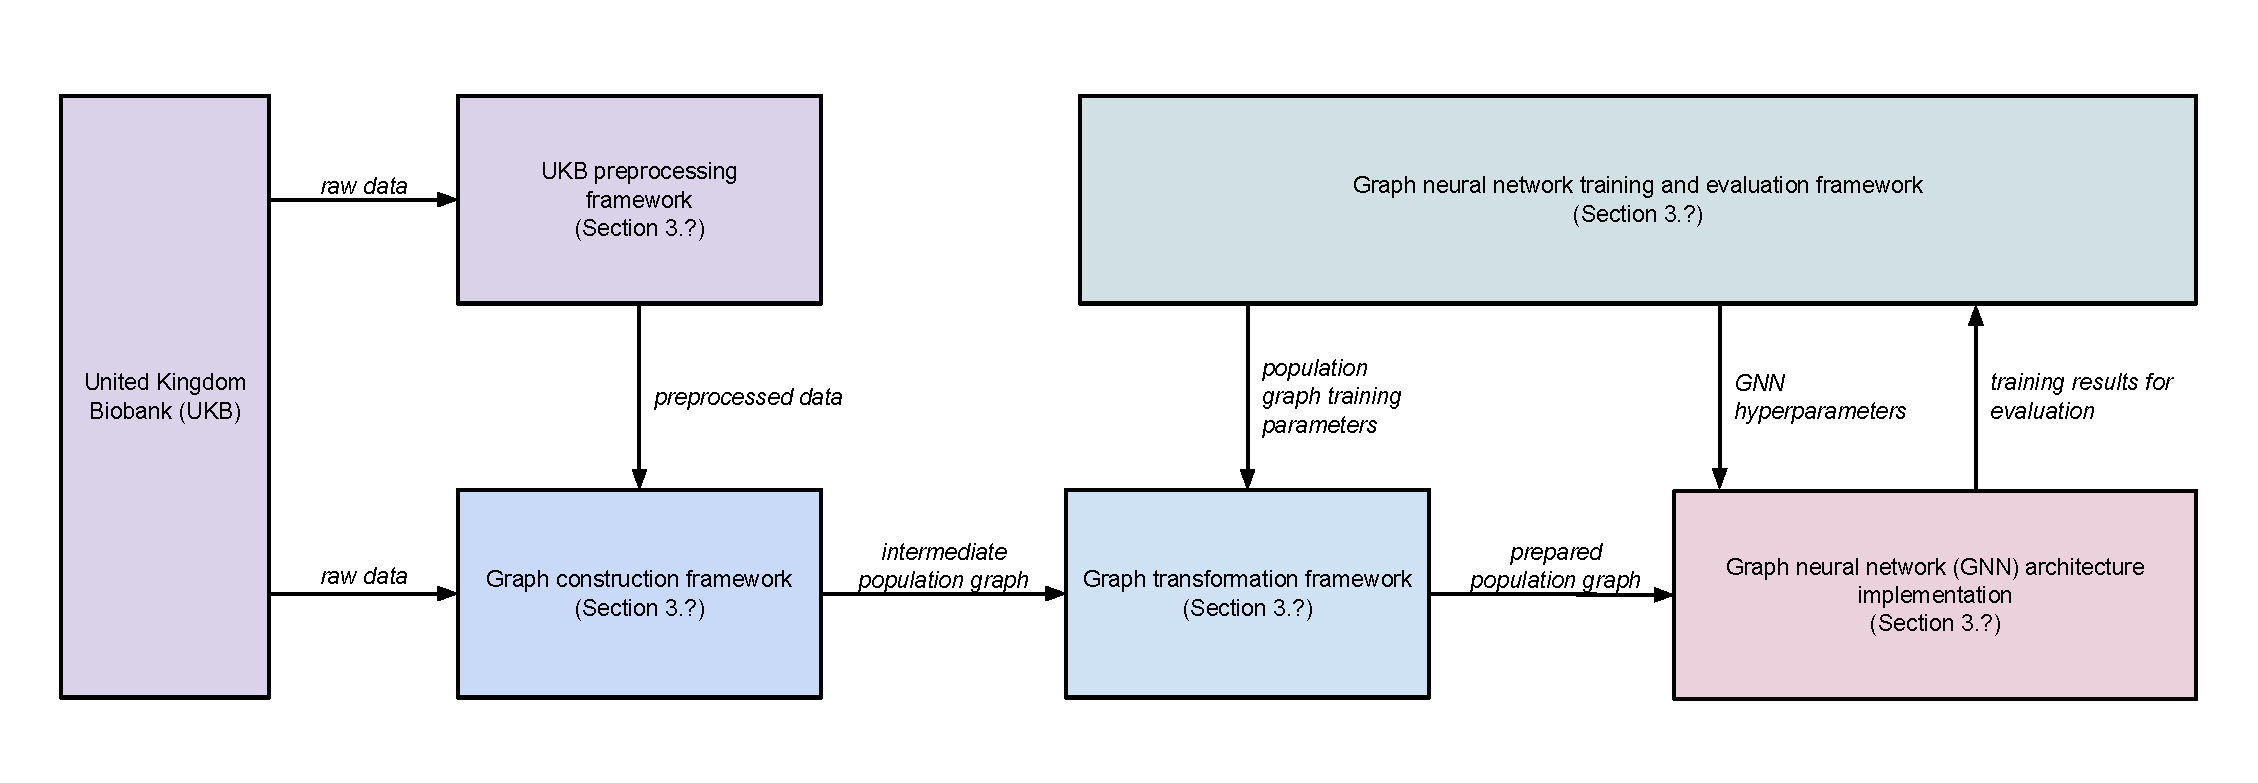
\includegraphics[width=\textwidth]{pipeline_overview.pdf}
    \caption{Overview of the key project components.}\label{pipeline-overview}
\end{figure}

This project can be divided into five key components, as illustrated in Figure~\ref{pipeline-overview}:
\begin{enumerate}
    \item Preparation of the United Kingdom Biobank (UKB) dataset;
    \item Intermediate population graph construction;
    \item Population graph transformation for training;
    \item Training on graph neural network architectures;
    \item Evaluation of the graph neural network performance.
\end{enumerate}

The work was split into these particular components so that each of them can carry out a single task independently of the other parts of the program, (other than the clearly defined input/output communication). This makes the overall project easier to implement, understand and extend in the future, generalising it to other datasets and preprocessing methods. 

This chapter will explain in detail the implementation behind each of the components.

\section{UKB preprocessing component}

The main function of the UKB preprocessing component is to prepare the raw or partially preprocessed UKB data for population graph construction. In particular, to improve the computational efficiency of operations later in the pipeline (potentially saving hours or days of computation time), this component preprocesses the data in a convenient form. This involves filtering the dataset, precomputing similarity matrices and functional connectivity matrices. The schematic diagram of these steps is shown in Figure~\ref{preprocessing-component}, which will be referred to throughout this section.

\begin{figure}[h]
    \centering
    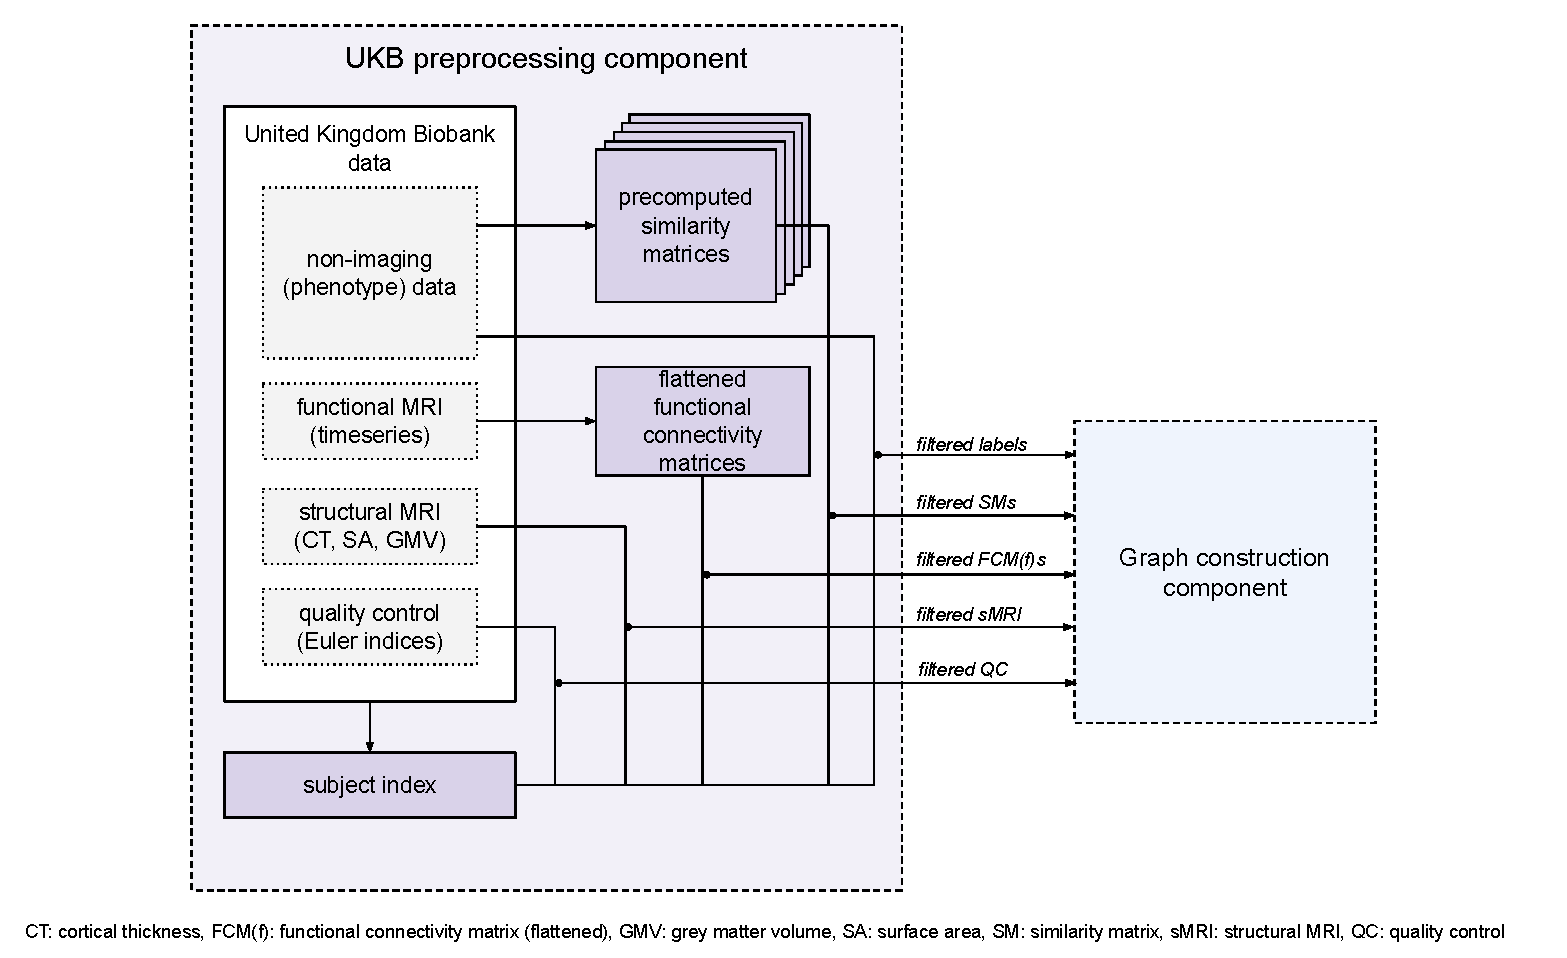
\includegraphics[width=\textwidth]{preprocessing_component.pdf}
    \caption{Overview of the UKB preprocessing component.}\label{preprocessing-component}
\end{figure}

\subsection{Cleaning the dataset}
The different modalities of the UKB data, shown in the white box in Figure~\ref{preprocessing-component}, have been provided separately from each other, with a small minority of subjects having the data available for some of the modalities but not others (for example due to data corruption or its retraction by the participant). To ensure consistent and smooth processing, the subjects with partially missing data (236 in total) have been excluded from further processing. The remaining 17,314 subjects with well-defined modalities have been collected into a \textit{subject index} (purple box on the bottom left), which was used to filter the data before its collection to the population graph construction component.

\subsection{Precomputing connectivity matrices}
The connectivity matrices involve computing pairwise correlations of 376 time-series (for 360 cortical and 16 subcortical regions) for every subject. With 20 gigabytes of raw timeseries data across over 17,000 subjects, this introduces a high computational overhead (a few hours on a CPU) if the matrices are computed on the fly as the graph is constructed. An additional inefficiency comes from the computation being repeated whenever a population graph that uses the functional data is constructed. To avoid this, the matrices are computed once for each subject, flattened and their lower triangles stored as \texttt{numpy} arrays as part of the preprocessing component.

% TODO could include the maths here?

\subsection{Precomputing similarity matrices}
The computation of pairwise similarity scores is quadratic in both time and space with respect to the number of subjects. Depending on the exact method how the similarity function is computed, a general-purpose (non-accelerated) processor might take hours or even days to process the entire dataset. This computation is also repeated whenever a graph is constructed, since the similarities per non-imaging metric do not change over different population graphs: the variation comes from different selections of subjects, non-imaging features, their relative weighting, and similarity thresholds.

The similarity matrices – one for each non-imaging feature in Table~\ref{table:phenotype-features} – have therefore been computed in advance. Unlike the functional connectivity data that is used directly for population graph node features (and therefore should avoid redundancy), the feature-wise similarity matrices are sliced and filtered depending on the selection of subjects. In this case it is more practical to store the full matrix, so that the integer indices into the similarity matrix directly correspond to the subject index in other components of the population graph data structure (see Section~\ref{section:population-graph-representation}).

Having computed the feature-wise similarity matrices, their linear combination for a full similarity score (by default adding matrices together and dividing the result by a constant) can efficiently make use of vectorised matrix operations.

For the \texttt{ICD10} metric, the subjects were considered to be \texttt{ICD10}-similar whenever they had at least one shared mental health or nervous system diagnosis, while two patients without any mental health or nervous system diagnoses were \textit{not} considered to be similar in order to avoid memory issues caused by a high number of edges (see Section~\ref{section:memory}). 

The similarity computation was vectorised in order to make use of accelerating hardware and reduce the compute time: for the boolean \texttt{ICD10}-lookup matrix $\mathbf{F}_{\text{ICD10}}$ with rows indexed by subjects and columns by relevant \texttt{ICD10} diagnoses, the pairwise similarity matrix $\mathbf{M}_{\text{ICD10}}$ computation corresponds to 

\begin{equation}
    \mathbf{M}_{\text{ICD10}} = \mathbf{1}\left[\mathbf{F}_{\text{ICD10}}^{\ }\mathbf{F}_{\text{ICD10}}^{\mathrm{T}} \geq 1\right]
\end{equation}

with the indicator function $\mathbf{1}[\cdot]$ applied element-wise.

For the remaining metrics (e.g. years of full-time education, \texttt{FTE}) there is only one integer or floating-point value per subject, with values  compared for equality. The computation is vectorised by exploiting \texttt{numpy}'s broadcasting operation\footnote{\url{https://docs.scipy.org/doc/numpy/user/basics.broadcasting.html}} that copies rows and columns as necessary for the matrix dimensions to match. For the vector of subject \texttt{FTE}s, $\mathbf{f}_{\text{FTE}}^{\mathrm{T}} \in \mathbb{R}^{N \times 1}$ and $\mathbf{F}_{\text{FTE}} = [\mathbf{f}_{\text{FTE}}^{\mathrm{T}} \cdots \mathbf{f}_{\text{FTE}}^{\mathrm{T}}] \in \mathbb{R}^{N \times N}$, \texttt{FTE}-similarity matrix is defined as

\begin{equation}
    \mathbf{M}_{\text{FTE}} = \mathbf{1}\left[\mathbf{F}_{\text{FTE}}^{\ } = \mathbf{F}_{\text{FTE}}^{\mathrm{T}} \right].
\end{equation}


% \[
% \begin{blockarray}{rccccc}
%  & b & c & d & e & f \\
% \begin{block}{r[ccccc]}
%   \text{UKB} & 1 & 1 & 1 & 1 & f \\
%   0 & 1 & 0 & 0 & 1 & g \\
%   0 & 0 & 1 & 0 & 1 & h \\
%   0 & 0 & 0 & 1 & 1 & i \\
%   0 & 0 & 0 & 0 & 1 & j \\
% \end{block}
% \end{blockarray}
%  \]


\section{Graph construction component}

The next stage of the pipeline involves constructing the ``intermediate representation'' of the population graph. The intermediate representation contains the graph topology and node features but is not prepared for training as it is not split into training, validation and test sets, and its features are not normalised. The two stages are separate because the same intermediate representation can be reused many times for different dataset splits and other training parameters without having to reconstruct the edges in $O(N^2)$ time for $N$ subjects. The steps for how the data is processed in this component is schematically visualised in Figure~\ref{graph-construction-component}.

\begin{figure}[h]
    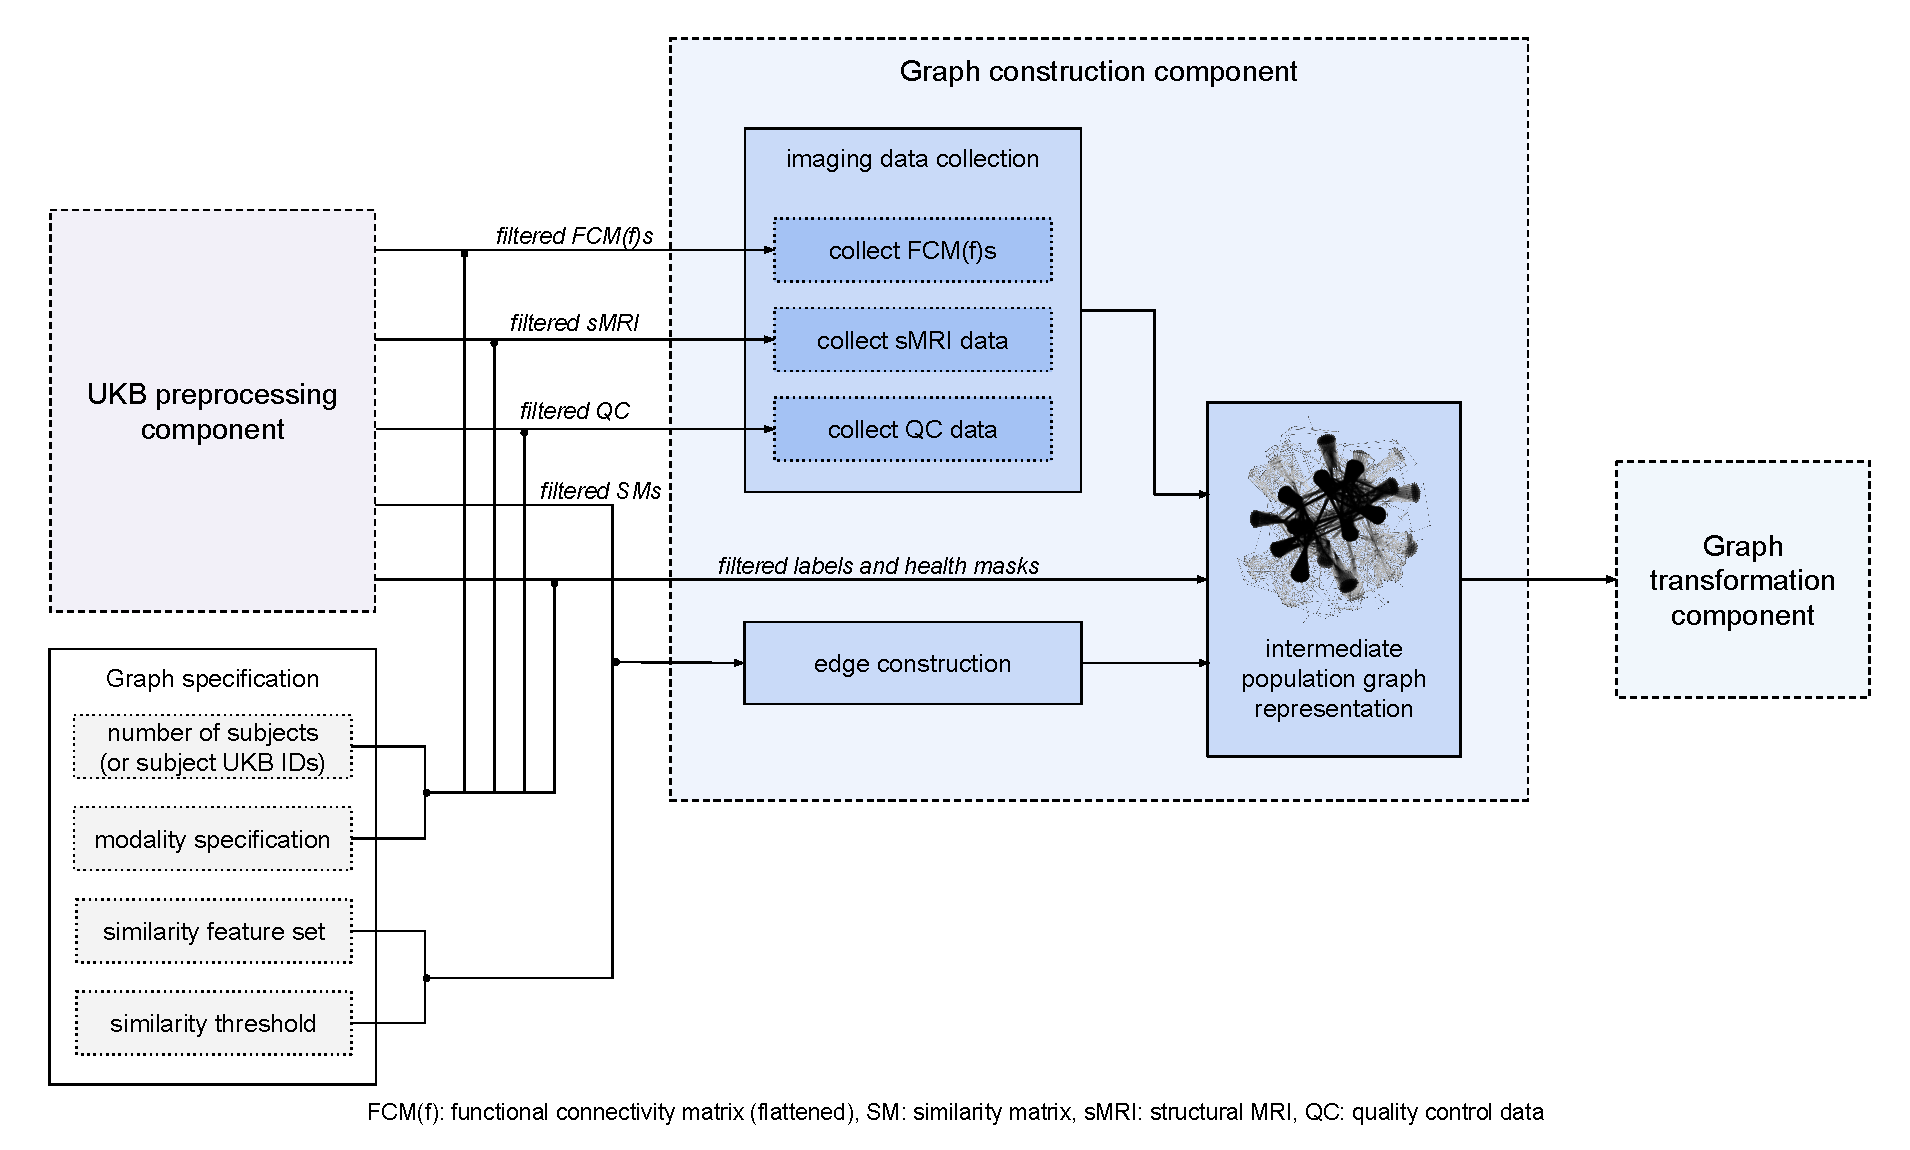
\includegraphics[width=\textwidth]{graph_construction_component.pdf}
    \caption{Graph construction component.}\label{graph-construction-component}
\end{figure}

\subsection{Inputs}
The inputs to the graph construction component can be categorised into four types as shown in the white box at the bottom left of Figure~\ref{graph-construction-component}:
\begin{enumerate}
    \item \textit{Modality specification} describes which of the neuroimaging modalities should be used as node features. This could be any combination of functional, structural and quality control data.
    \item \textit{Subject specification} takes in the number of (randomly selected) subjects that should be used to create the graph, or a list UKB identifiers for a graph containing a particular set of subjects. If no such parameter is provided, then all available data (filtered by the subject index described in the previous component) is used for population graph construction.
    \item \textit{Similarity specification}. 
    In its default implementation, the similarity score is computed as the average over a set of similarity features $\{M_1, \dots, M_n\}$ (see Equation~\eqref{eq:similarity}), in which case it is sufficient to specify the similarity feature set to be used. An \textit{extension} to this is to accept an arbitrary linear combination of various similarity features, allowing for much richer similarity metrics. 
    \item \textit{Similarity threshold}. A number $\mu \in [0,1]$ defining the threshold for the similarity metric above which an edge will be added to the graph (see Equation~\eqref{eq:similarity-threshold}).
\end{enumerate}


\subsection{Imaging data collection}

Based on the subject and modality specification, the relevant imaging data is collected from the raw UKB files (first filtered by subject index) and stored in the intermediate representation as a \textit{dataframe} (\texttt{pandas.DataFrame} object) indexed by UKB subject identifier. This is represented by the connections between UKB preprocessing component, graph specification and the blue imaging data collection box in Figure~\ref{graph-construction-component}. 

If a particular modality is unused, the dataframe stored is empty.

\subsection{Edge construction}

The edge construction component uses the subject specification, similarity specification, and the filtered similarity matrix data to find the similarity scores for each pair of subjects. Whenever the similarity score between two subjects exceeds the threshold, an undirected edge is added to the population graph. The edges are stored in a \textit{tensor} (\texttt{torch.tensor}), which is a PyTorch datatype for multi-dimensional matrices\footnote{\url{https://pytorch.org/docs/stable/tensors.html}}.

\subsection{Brain health mask computation}

Due to the nature of the brain age problem, the machine learning model can only be trained on subjects with healthy brains, although the population graph may contain both healthy and non-healthy subjects. The \textit{brain health mask} is therefore computed to determine which subjects can be used to train the model and which cannot. In particular, non-healthy subjects are not included in loss function computation, so that the direction of parameter update depends on healthy subjects only (though the parameters are updated for the entire graph). As a result, the predicted labels are available for both healthy and non-healthy subjects, but the use of a brain health mask ensures that the prediction corresponds to the brain age rather than chronological age, as discussed in Section~\ref{brain-age-estimation}.

In this project, the brain health is approximated by the absence of diagnoses related to mental health or nervous system disorders, defined by the \texttt{ICD10}-similarity metric (see Table~\ref{table:phenotype-features}).

\subsection{Population graph representation}
\label{section:population-graph-representation}

The population graph is stored in an extended \texttt{torch\_geometric.Data} object\footnote{\url{https://pytorch-geometric.readthedocs.io/en/latest/modules/data.html}}, with its most important fields listed in Table~\ref{table:population-graph}. The intermediate population graph representation has all of its entries defined except for the feature vector \texttt{x} and the training, validation and test masks.

\setlength{\LTpost}{0pt}
\renewcommand{\arraystretch}{1.25}
% \begin{table}[]
%     \caption{The population graph data structure (excludes helper or utility fields).}\label{table:population-graph}
%     \centering
%     \begin{tabular}{lp{0.2\textwidth}p{0.5\textwidth}}
%         \hline
\begin{center}
\begin{longtable}[]{lp{0.175\textwidth}p{0.475\textwidth}}
    \caption{The population graph data structure (excludes helper or utility fields).}\label{table:population-graph}\\
    \hline \textbf{Field name} & \textbf{Type} & \textbf{Description} \\
    \hline
    \endfirsthead
    \multicolumn{3}{c}%
    {\tablename\ \thetable\ -- \textit{Continued from previous page}} \\
    \hline
    \textbf{Field name} & \textbf{Type} & \textbf{Description} \\
    \hline
    \endhead
    \hline \multicolumn{3}{r}{\textit{Continued on next page}} \\
    \endfoot
    \hline
    \endlastfoot
    % \texttt{num\_nodes} & long & Number of nodes (subjects) in the population graph. \\
    \texttt{subject\_index} & string array & UKB identifiers of the subjects. Stored in the same subject order as training masks, feature and label tensors; corresponds to the edge start and end values. \\
    \texttt{edge\_index} & $2\times 2|E|$ \hfill\newline long tensor & \texttt{edge\_index}$[0][i]=s_v$ and \hfill \newline \texttt{edge\_index}$[1][i]=s_w$ indicate a directed \hfill \newline edge $s_v \leadsto s_w$. To represent the undirected edge $(s_v, s_w) \in E$, the second directed edge $s_w \leadsto s_v$ is added. \\
    \texttt{functional\_data} & dataframe & Row-indexed by subject with columns containing the flattened functional connectivity matrix entries. Empty if no functional data is used in the population graph. \\
    \texttt{structural\_data} & dictionary of \hfill \newline dataframes & Dictionary is indexed by the structural data modality, in this case cortical thickness, surface area, and grey matter volume. The corresponding dataframes are row-indexed by subject with columns containing the features of the relevant structural data modality. The dataframes are empty if no structural data is used. \\
    \texttt{quality\_control\_data} & dataframe & Row-indexed by subject with the columns containing Euler indices for the left and right hemispheres of the brain. Empty if no quality control data is used. \\
    \texttt{x} & $N \times F$ \hfill\newline float tensor & \textit{Unused at the intermediate stage.} Contains the full normalised feature vector (of $F$ features) for every graph node (subject). \\
    \texttt{y} & $N \times 1$ \hfill \newline float tensor & Contains the labels of training data, in this case chronological age. \\
    \texttt{brain\_health\_mask} & boolean array & \texttt{True} indicates that the subject has a healthy brain and can be used for training, and \texttt{False} otherwise. \\
    \texttt{train\_mask} & boolean tensor & \textit{Unused at the intermediate stage.} \texttt{True} if the subject belongs to the training set, and \texttt{False} otherwise. \\
    \texttt{validation\_mask} & boolean tensor & \textit{Unused at the intermediate stage.} \texttt{True} if the subject belongs to the validation set, and \texttt{False} otherwise. \\
    \texttt{test\_mask} & boolean tensor & \textit{Unused at the intermediate stage.} \texttt{True} if the subject belongs to the test set, and \texttt{False} otherwise.
    % \end{tabular}
\end{longtable}
\end{center}

\section{Graph transformation component}

The graph transformation component is responsible for preparing the intermediate population graph representation for training by defining its normalised, concatenated feature vector as well as training, validation and test masks. The schematic diagram representing the population graph transformations in this component is shown in Figure~\ref{graph-transformation-component}.

\begin{figure}[h]
    \centering
    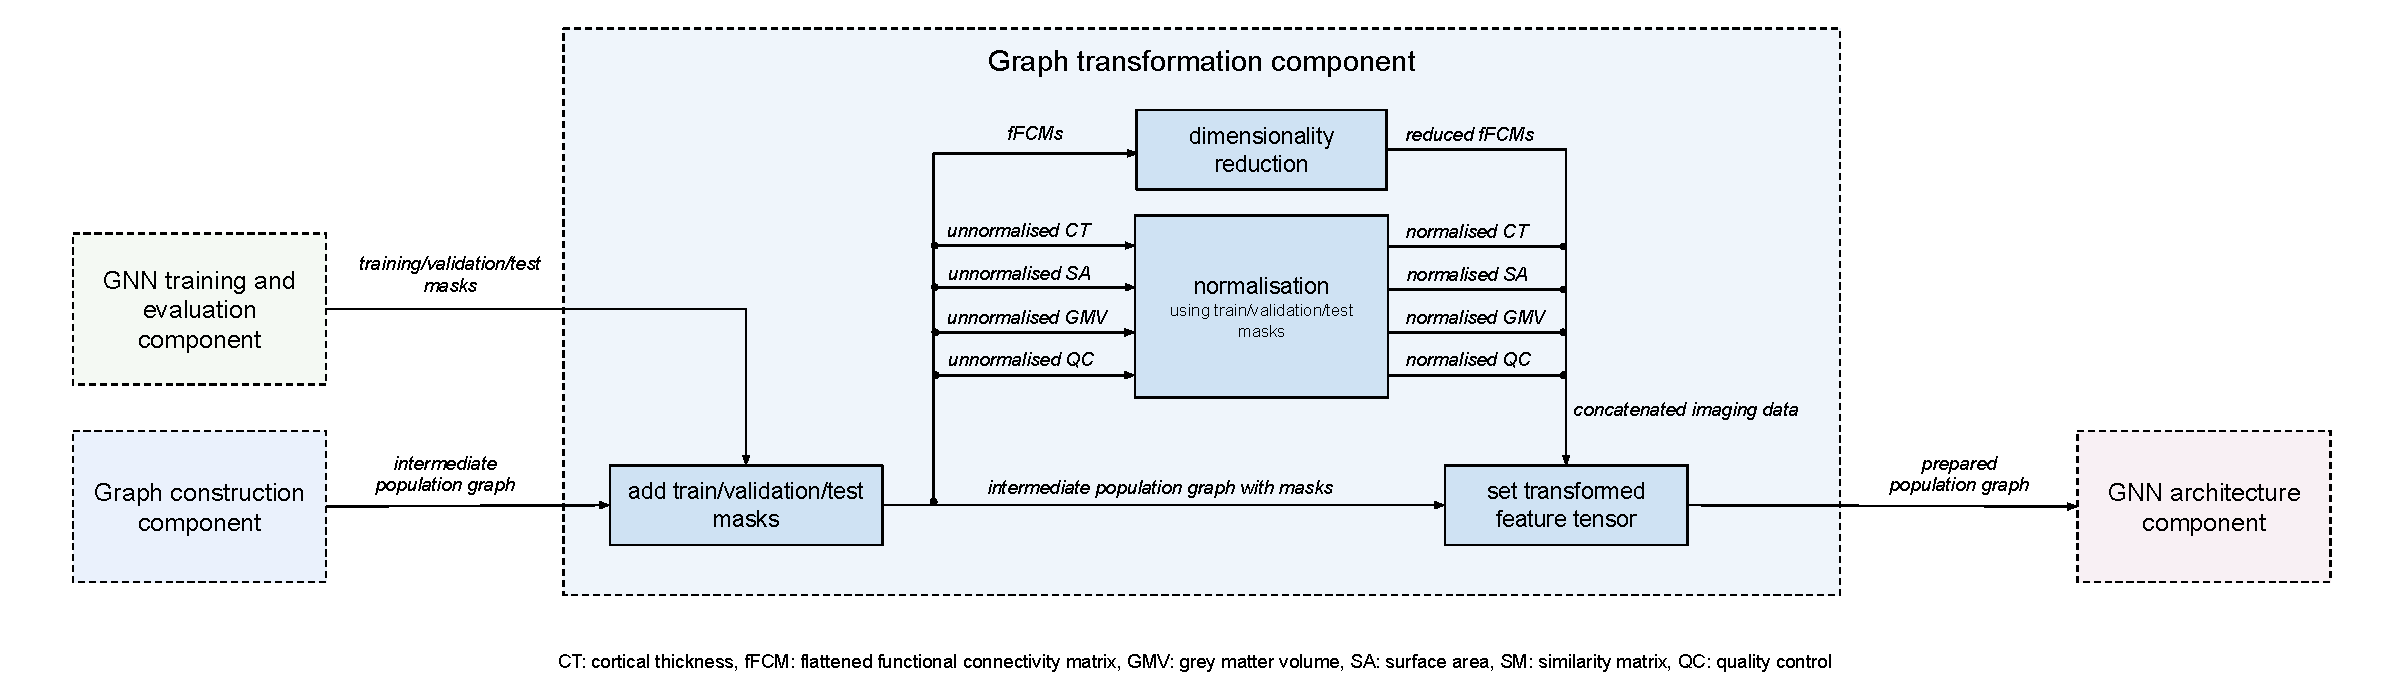
\includegraphics[width=\textwidth]{graph_transformation_component.pdf}
    \caption{Graph transformation component.}\label{graph-transformation-component}
\end{figure}

\subsection{Setting the training masks}
The first operation for preparing the population graph for training involves setting the \texttt{train\_mask}, \texttt{validation\_mask} and \texttt{test\_mask} fields of the intermediate population graph data structure (see Table~\ref{table:population-graph}). 

Following the brain age estimation method (Section~\ref{brain-age-estimation}), the masks are intersected with the \texttt{brain\_health\_mask}. Similarly to the reasoning behind the brain health masks, the three training masks are used to determine which nodes should be used to compute the loss function during various stages of training. For example, the model parameters are only updated based on the loss function for the subjects filtered with the \texttt{training\_mask}, and validation loss is computed only for the subjects filtered with the \texttt{validation\_mask}.

\subsection{Functional connectivity matrix dimensionality reduction}
The flattened functional connectivity matrix results in over 75,000 features per patient. Since the population graph cannot be split into parts and during training must be kept entirely in memory, along with all model parameters, this quickly runs into memory issues when the entire dataset is used. To mitigate this issue, some techniques may be applied to reduce the dimensionality of functional data. This project uses principal component analysis (PCA) as the dimensionality reduction technique of choice as it is one the simplest to implement. When the functional data is used to construct the population graph, PCA transformation is fitted to the training set as specified by the \texttt{training\_mask}, and the same transformation is applied to the remaining subjects. This dimensionality reduction technique is optional, and it is possible to define how many principal components should be kept after the transformation, to control the information loss.

\subsection{Structural MRI and quality control data normalisation}
Next, the raw features stored under \texttt{structural\_data} and \texttt{quality\_control\_data} are normalised to be in the range between $-1$ and $1$ with mean 0. Similar to the previous section, to avoid data leakage standard scaler is fitted to the training set only (as specified by the \texttt{training\_mask}) and then applied to the validation and test sets. A separate transformation is applied to each structural data modality (cortical thickness, surface area, grey matter volume) and the quality control modality.

\subsection{Setting the transformed feature tensor}
The transformed functional, structural and quality control features are concatenated together into a single tensor, which is assigned to \texttt{x} in the population graph data structure (Table~\ref{table:population-graph}). This completes graph transformation for training.

Since the original neuroimaging dataframes and brain health masks are kept unchanged in the data structure, the same population graph can be prepared for, say, a different training fold by simply going through the transformation component again but with a different training mask set, which will reset the values in the corresponding population graph fields.

\section{GNN architecture component}
% gcn_train(graph, device, n_conv_layers=0, layer_sizes=None, epochs=3500, lr=0.005, dropout_p=0, weight_decay=1e-5,
% log=True, early_stopping=True, patience=10, delta=0.005, cv=False, fold=0, run_name=None,
% min_epochs=1000):

The graph neural network component contains the implementations for the graph neural network (GNN) architectures used in this project: the graph convolutional network (GCN, Section~\ref{training-gcn}) and the graph attention network (GAT, Section~\ref{training-gat}). The networks are implemented as two PyTorch modules called \texttt{BrainGCN} and \texttt{BrainGAT}, which extend the base \texttt{BrainGNN} module. Table~\ref{table:braingnn} presents the parameters used to define a \texttt{BrainGNN} instance. \texttt{BrainGCN} and \texttt{BrainGAT}  have identical structure except that the \texttt{conv\_type} parameter is instantiated to \texttt{GCN} and \texttt{GAT} respectively, and the convolutional layers are set to either \texttt{torch\_geometric.nn.GCNConv} or \texttt{torch\_geometric.nn.GATConv} layers, both implemented in PyTorch Geometric library.


\begin{center}
    \begin{longtable}[]{p{0.275\textwidth}p{0.175\textwidth}p{0.475\textwidth}}
        \caption{The parameters for the \texttt{BrainGNN} module.}\label{table:braingnn}\\
        \hline \textbf{Parameter} & \textbf{Type} & \textbf{Description} \\
        \hline
        \endfirsthead
        \multicolumn{3}{c}%
        {\tablename\ \thetable\ -- \textit{Continued from previous page}} \\
        \hline
        \textbf{Parameter} & \textbf{Type} & \textbf{Description} \\
        \hline
        \endhead
        \hline \multicolumn{3}{r}{\textit{Continued on next page}} \\
        \endfoot
        \hline
        \endlastfoot
        
        \texttt{conv\_type} & string & Indicates the type of graph convolutional layer to be used (graph convolution or graph attentional layer). \\
        \texttt{layer\_sizes} & integer array & Lists the number of units in every hidden layer. The length of the array corresponds to the total number of hidden layers. \\
        \texttt{n\_conv\_layers} & integer & Number of convolutional layers. Must be in range $[0, \text{\texttt{layer\_sizes}}]$. The sizes of those layers are determined by the first \texttt{n\_conv\_layers} values of the \texttt{layer\_sizes} and \texttt{n\_node\_features} parameters. \\
        \texttt{num\_node\_features} & integer & Indicates the number of input features. \\ 
        \texttt{dropout\_p} & float & The probability of ignoring the node in a hidden layer. Used as a regularisation technique to reduce overfitting.
    \end{longtable}
    \end{center}

TODO perhaps simplify this? I don't know which parts to cut out of this for it to be clearer – what's unnecessary? I could also write pseudocode but not sure where it falls in the clarity vs professional spectrum. I could also delete the initialisation as I still plan to make a diagram for it – just not sure how to visualise how the \textit{array of parameters} is used.

\bigskip
\begin{code}
\caption{Simplified code snippet for \texttt{BrainGNN} instantiation and training.}
\label{listing:braingnn}
\medskip
\inputminted[frame=bottomline, linenos, breaklines=true, numberblanklines=false, style=colorful]{python}{code/brain_gnn_snippet.py}
\end{code}

Listing~\ref{listing:braingnn} shows how the order in which the layers are combined in the \texttt{BrainGNN} architecture, given the parameters in Table~\ref{table:braingnn}. I chose the hyperbolic tangent $\tanh(\cdot)$)as the non-linearity (activation function) between each layer because the inputs and values in neurons may be negative, in which case the other popular activation functions such as $\mathrm{ReLU}(\cdot)$ would have an undesirable asymmetric response. The \textit{dropout} layers have been added between the every fully connected layer as a regularisation technique: with probability \texttt{dropout\_p}, a unit in the layer is ignored at training time (its weight is zeroed) with the hope that the neural network will not rely on any particular node when predicting age, learning more robust features.


\section{GNN training and evaluation component}

\begin{figure}[]
    \centering
    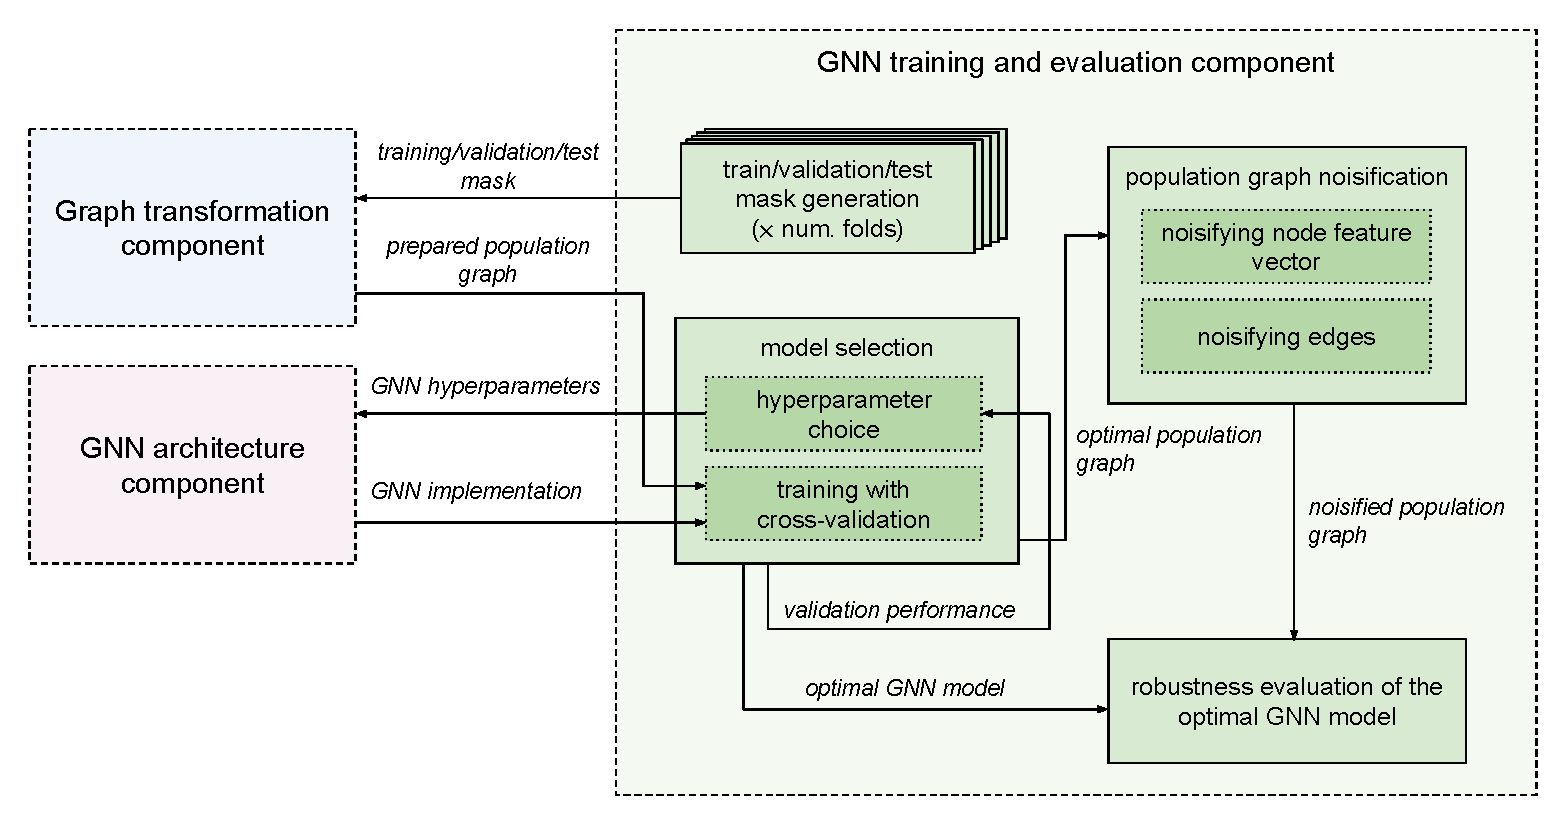
\includegraphics[width=\textwidth]{gnn_training_eval_component.pdf}
    \caption{Graph neural network training and evaluation component.}\label{gnn-training-eval-component}
\end{figure}

The main function of the GNN training and evaluation component is to select the best combination of population graph and GNN hyperparameters for each of the GCN and GAT architectures and report the results of the best model. A further \textit{extension} to this is the \textit{robustness evaluation} component, where robustness in this project is defined as the rate of the predictive power drop as noise is added to the population graph nodes or edges. The schematic overview of the GNN training and evaluation component is shown in Figure~\ref{gnn-training-eval-component}.


\subsection{Model selection}
% Hyperparameter tuning, weights and biases

With a high range of population graph modality (functional, structural, quality control data), similarity metric (Table~\ref{table:phenotype-features}), similarity threshold, as well as the GNN construction (Table~\ref{table:braingnn}) and training parameter (such as learning rate and number of epochs) choices, the search space for the best performing model is vast and it may be out of scope of this project to find the best fitting model.

TODO  I don't know whether the department likes something written in the first person. But I think is the first time you use this, so maybe doublecheck or think about it
The search space might be even bigger considering that I do not use all the possible non-imaging features in Table~\ref{table:phenotype-features} and there might be more confounders. There could be more similarity functions and the relative weights for each similarity feature – the subject's sex is probably more important than how many years they had of full-time education, for example. The UK Biobank has 768 non-imaging features per patient – it's out of scope to select the best ones and their relative weights and thresholds, especially having no neuroscience expertise etc\dots


Nonetheless I selected the set of features that I felt were the most important and carried out the hyperparameter tuning over the selected ranges of features.

\subsubsection{Mitigating memory constraints}
\label{section:memory}
The biggest constraint in training the population graphs was GPU memory (which accounting for intensive GPU usage in the laboratory was up to 5-8 gigabyte models, and often even 1-3 gigabyte models). This especially affects the population graph training since in this case, to train on the full dataset, the entire graph of more than 17,000 subjects must be in memory at once due to subject similarity connections, and unlike in most models that have individual independent examples, the population graph cannot be trivially split into smaller batches. At the same time, GCN and GAT are known to be memory-intensive models.
TODO reference
I wanted to use the entire dataset (
TODO why? – because the (quality of) data is often more important than the model, reference?),
which meant that I had to constrain my model and population graph structure selection instead. I constrained it as follows:

TODO "I decided" is def not a good wording here... try to make it just a normal, direct consequence from what you've read in the literature
\begin{enumerate}
    \item Having referred to the literature on brain age estimation, I decided that high-dimensional functional imaging data modality is less promising than structural imaging data modality, while adding a lot of extra features per patient (over 78,000). Functional imaging data is never used alone (especially because it's already very much an estimate of how the brain works and includes a lot of oversimplified assumptions to how the brain is connected, and if used, it is generally to only complement structural data). Dimensionality reduction is possible, but from experience from the practical work of my Data Science Unit of Assessment, PCA, for example, cutting out half of the low-variance principle components can even worsen the predictive power and training time of the model instead of improving it. While the support for those techniques is implemented – which indeed was the goal of this project to support it if it is needed – it was not used in training.
    \item The model size was fixed to a fairly shallow network with a small number of units (
        TODO give the actual architecture). 
        The learning rates were decreased and epochs increased to compensate for the smaller number of training parameters.
    \item I fixed the set of possible population graph types and the similarity thresholds (
    TODO see full list in Appendix ?). 
    From running some initial models I found that feasible similarity thresholds are all above 0.6, and even 0.7 or 0.8 often cause problems. 
\end{enumerate}


Hyperparameter search was restricted to only use the default similarity metrics for a more consistent training and because it is not clear how each metric should be weighted. The intent behind supporting this is the capability for a neuroscientist or another professional with domain knowledge to design their own good similarity metric – which has been implemented as an \textit{extension} to my original success criteria. Otherwise the weighting would be very arbitrary and increase the search space even more. As someone without much neuroscience domain knowledge I went for the simplest way of combining the metrics for this training procedure.

TODO in general lessons learnt and things for the future is that the memory issues and uninformed similarity metric and GNN architecture decisions severely restricted my hyperparameter search space, and very likely missed out on promising models with good test set performance. When I have time I would love to explore more hyperparameter options, consulting Dr Bethlehem and other experts on what other non-imaging features to include, how to combine them, how to adjust the architecture, and test new models on new data, for example on the recent UKB update which I did not have access to before, or some entirely new dataset. Alternatively, I could try training higher range of model hyperparameters on subsets of the UKB dataset, e.g. on 2,000-brain graphs which would decrease the parameters but allow for better exploration of the similarity matrix and GNN architecture possibilities.


\subsubsection{Hyperparameter tuning}
TODO is this implementation or evaluation? I feel like I could move it to evaluation so that I can show the results over each fold and how I selected them, not sure.

With the above GNN hyperparameter and population graph parameter restrictions due to memory constraints, I optimised the remaining hyperparameters using Bayesian optimisation strategy using the \textit{Sweeps} tool provided by the \textit{Weights~\& Biases}~\cite{wandb} (\texttt{wandb}) machine learning tracking and optimisation framework. 

TODO this is simplified – not sure how much do I want to explain the Gaussian processes etc.
Having integrated the training with the \texttt{wandb}, the framework would automatically suggest and test the best hyperparameter combinations it believes are the most likely to optimise the performance metric of choice, which in my case was to minimise the average cross-validation mean squared error (MSE). 

I ran the sweeps for both GCN and GAT models for at least 100 runs (most of them still unsuccessful due to the memory constraints) until the models started to converge to similar performance that could not be improved with new hyperparameters, and selected the best one for each architecture based on the lowest MSE.

TODO The hyperparameters tuned, their distributions and value ranges tuned can be found in Appendix ?.

TODO where to include this??? The models are trained using early stopping with patience of 100 and delta 0.005. This means that the training stops if the validation set MSE does not decrease by at least 0.005 in 100 consecutive epochs, at which point the model is reverted back to the state that gave the best validation set score). Otherwise, the models are trained for at least 1000 epochs and for a maximum of 7500 epochs.

\subsubsection{Cross-validation}
The subjects are first split into the 90\% training and 10\% hold-out test set, stratifying by subject age and sex. The test set will be used to evaluate a single selected model. 

The remaining data was used for model selection (hyperparameter tuning). The models were trained with five-fold cross-validation, so that the training data split into five folds with 90\% true training and 10\% validation subjects. Therefore for a given set of hyperparameters five models are trained, and the model's overall performance is estimated using the average mean squared error across the folds as well as the variation in performance. 

As the hyperparameter tuning converges, the most promising model is selected to be tested on the hold-out test set. The metrics usually used to evaluate the models performing a regression task are Pearson's correlation $r$ and coefficient of determination $r^2$.

\subsection{Robustness measurement}


The standard performance metrics $r$ and $r^2$ tracked and logged with training.

Describe the additional graph transformation stages which add noise to node features/edges.


\section{Repository overview}
% The repository overview should be around one page in length and should describe the high-level structure of the source code found in your source code Repository; ... could be implemented as a table with folders/file names and the functionality implemented in those files

